\section{Place Recognition Algorithm}
\label{sec:chap_slam_algo}

While there is quite a few articles presenting place recognition algorithms using different sensors (e.g. cameras, \gls*{gps}), the literature of such algorithms based solely on \gls*{3d} data is limited. For our place recognition analysis, we choose to evaluate on our datasets the state-of-the-art algorithm (at the time of the experiments) developed by \citet{Steder2011b}. The full details of the technique are presented in the article. However for the sake of this document, we will first describe some fundamental concepts used for place recognition in Section~\ref{ssec:chap_slam_basics} and then we will give an overview of the Steder algorithm itself in Section~\ref{ssec:chap_slam_algo}.


\subsection{Fundamental Concepts}
\label{ssec:chap_slam_basics}

\subsubsection{Feature Keypoints and Descriptors}
\label{ssub:feature_keypoints_and_descriptors}

The first step to determine whether or not a place has been visited before by the robot, is to convert the data into a more convenient format for identification. The generally adopted representation is a vector of real numbers, called descriptor. A descriptor can be global, meaning that it tries to capture information about the whole sample, or local, meaning that it does the same but only for a specific subregion of the sample. When using local descriptors, it is first required to determine the keypoints around which the descriptors will be extracted. These keypoints can be at pre-determined and fixed locations (e.g. division in a simple grid) or selected using more refined algorithms. A common practice is to choose keypoints in regions of high gradient (e.g. edges, corners), since these region generally contains more information than smooth surfaces. Note that for simplicity, we might use the term \textbf{features} as a more general term for keypoints and their respective descriptors in the remainder of this document.

The concepts of keypoints and descriptors originate from the computer vision literature, but they have been adapted for \gls*{3d} data. Some popular examples of features for both type of data are shown in Table~\ref{tab:chap_slam_features_examples}. Note that some algorithms propose solutions for both keypoints detection and descriptors (e.g. SIFT, NARF), however it is not mandatory to use them together as any combination is generally valid. While features are different, they were all developed with the same goals in mind:
\begin{itemize}[label=$\bullet$,noitemsep,topsep=0pt]
    \item Distinctiveness: each feature should be easily differentiable with respect to other.
    \item Repeatability: the feature values should be stable under changes including:
        \begin{itemize}[label=$\circ$,noitemsep,topsep=0pt]
            \item Transformations: rigid transformation for point clouds and projective transformation for images, but also changes of the pose of the objects and the viewpoint.
            \item Noise: small variations in measurements (range/intensity) and occasional erroneous values (points/pixels).
            \item Resolution: the amount of points or pixels representing a given area.
        \end{itemize}
\end{itemize}

\begin{table}[H]
    \centering
    \begin{tabular}{@{}llll@{}}
        \toprule
        \textbf{Type of data}  & \textbf{Keypoint/descriptor} & \textbf{Name}               & \textbf{Reference} \\
        \hline
        Image                  & Keypoint                     & Harris and Stephens corners & \cite{Harris1988}  \\
        Image                  & Both                         & SIFT                        & \cite{Lowe2004}    \\
        Image                  & Both                         & SURF                        & \cite{Bay2006}     \\
        \gls*{3d}              & Descriptor                   & FPFH                        & \cite{Rusu2009}    \\
        \gls*{3d}              & Both                         & ISS                         & \cite{Yu2009}      \\
        \gls*{3d}              & Descriptor                   & SHOT                        & \cite{Tombari2010} \\
        \gls*{3d}              & Both                         & NARF                        & \cite{Steder2011a} \\
        \bottomrule
    \end{tabular}
    \caption{\todo{Might just put image examples in the text, find better layout ? Add info ?} Examples of popular descriptors and keypoints detectors for images and \gls*{3d} data. Some \gls*{2d} keypoints have been adapted for \gls*{3d} such as Harris and Stephens and SIFT.}
    \label{tab:chap_slam_features_examples}
\end{table}

\subsubsection{NARF Features and Range Image}
\label{ssub:NARF Features and Range Image}

For our place recognition analysis, we choose to use the NARF keypoints and descriptors. The computation of those features requires a preprocessing step, which consist in converting the point cloud into a range image. We will see in Section~\ref{ssec:chap_slam_algo} that the place recognition algorithm rely on this \gls*{3d} representation to determine a matching score between scans.

Overall, range images are spherical projection of the points from the center of the sensor, but some constraints must be satisfied for its creation. Firstly, there must be no missing points in the scan. Since this is not satisfied for our data, all missing points are considered as far range (i.e. the maximum range of the sensor). In addition, the resolution has to be adjusted so that each pixel of the resulting range image covers the same angular resolution vertically and horizontally. Finally, this conversion requires the acquisition to originate from a single view point and to have a single range value per pixel. It is therefore not possible to use point clouds acquired with multi-echoes \gls*{lidar}s or produced by merging multiple scans. Fortunately, the latter constraint is met in our datasets. Examples of range images can be seen in Figure~\ref{fig:chap_slam_range}.

The converted scans has a dense and uniform representation that can be advantageously processed like greyscale images. Using these range images, NARF features are able to differentiate edges that are part of the boundary of objects as opposed to edges that are produced by occlusions, which is not possible using point clouds directly. This is useful in highly occluded environments such as forest, where edges caused by occlusions can generate meaningless features. This in turn leads to a poor representation of the environment, which can reduce the place recognition performance.


\begin{figure}[H]
    \centering
    \subfloat[]{\label{fig:range_building}}{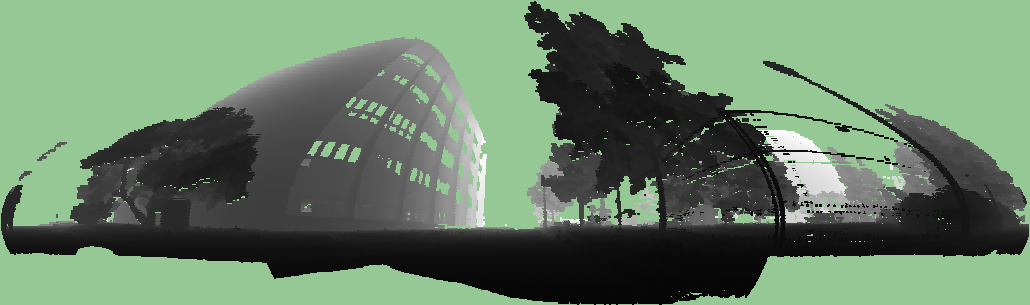
\includegraphics[width=0.995\linewidth]{img/chap_slam/range_building01.png}}\\
    \subfloat[]{\label{fig:range_forest}}{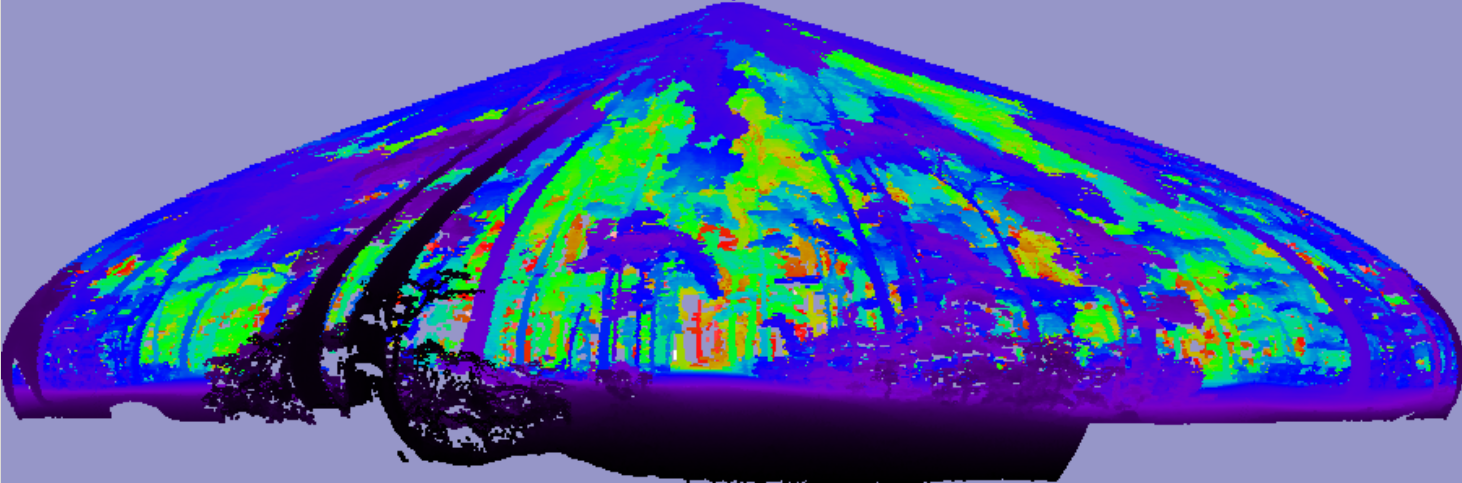
\includegraphics[width=0.995\linewidth]{img/chap_slam/range_forest01.png}}
    \caption{Examples of range images for the structured dataset \protect\subref{fig:range_building} and the unstructured dataset \protect\subref{fig:range_forest}. Note that the objects look distorted due to the projection on the plane and that the background color corresponds to the areas without laser return.}
    \label{fig:chap_slam_range}
\end{figure}

\subsubsection{Scans Comparison}
\label{ssub:scans_comparison}

The last item we need to discuss in this subsection is the method used to compare two scans. This task rely on the similarity between descriptors, which can be computed using a simple distance metric (e.g. Euclidean distance, cosine distance). For global descriptors that represent an entire scan, this is a simple and computationally inexpensive process. A major drawback of such comparison approach is the high sensitivity to local changes. Although methods based on local descriptors require more computation, they generally yield more robust results. As we will see, because a scan is made up of several local descriptors, there are different techniques for comparison.

A popular solution is to convert this set of local features into a single \gls*{bow}\todo{cite?} and then use this new representation for comparison. The concept of \gls*{bow} was first used for documents classification. In this context, \gls*{bow} represented a document by a vector of occurrence counts of a vocabulary. In our case, the amount of descriptors made up of real numbers is infinite and therefore cannot be used directly as words. The solution to this problem is to use a clustering algorithm such as k-means\todo{cite?} to create groups that will represent words, process known as quantization. The vocabulary is generally created in advance using a large collection of local descriptors gathered under similar conditions. Because no labels are required for this step, this operation does not demand a lot of human work. The representation in words avoids having to compare the descriptors according to their distance in the space of descriptors. One possible drawback is that it remove all information regarding to geometric configuration of keypoints in the scans, which might induce unwanted aliasing. This is a rather general representation with which the comparison is relatively fast to compute.

Another approach to compare \gls*{3d} scans consist in finding local descriptors correspondences and checking if there is a valid transformation that aligns these. The vectors of real numbers representing the features (i.e. the descriptors) will never be exactly the same from one scan to another, but a simple solution is to use the nearest neighbor as the correspondence. Unfortunately, this does not take into account that several descriptors may have no valid match due to background clutter or change in the view point. \cite[Section 7.1]{Lowe2004} describes how to remove most of the false matches by comparing the distance of the closest neighbor to that of the second-closest neighbor. Using this ratio, only matches that have the closest neighbor significantly closer than the closest incorrect match will be used, therefore improving reliability.

Once the corresponding descriptors between two scans have been identified, they are used to determine if there is a valid rigid \gls*{3d} transformation that align the underlying keypoints. This step also requires a criteria on the number (or ratio) of features correctly aligned, thereby identifying the scans as originating from the same place or not. This is generally achieved using the RANSAC algorithm\todo{cite?}. This second technique is more computationally expensive, but is also more discriminative. Additionally, it provides relative pose between scans, which is not possible using global descriptors or \gls*{bow}s. This relative pose can, for example, be used to determine odometry or create a map. Figure~\ref{fig:chap_slam_features_correspondences} shows keypoints from two scans of our dataset, as well as examples of correspondences.

\begin{figure}[H]
    \centering
    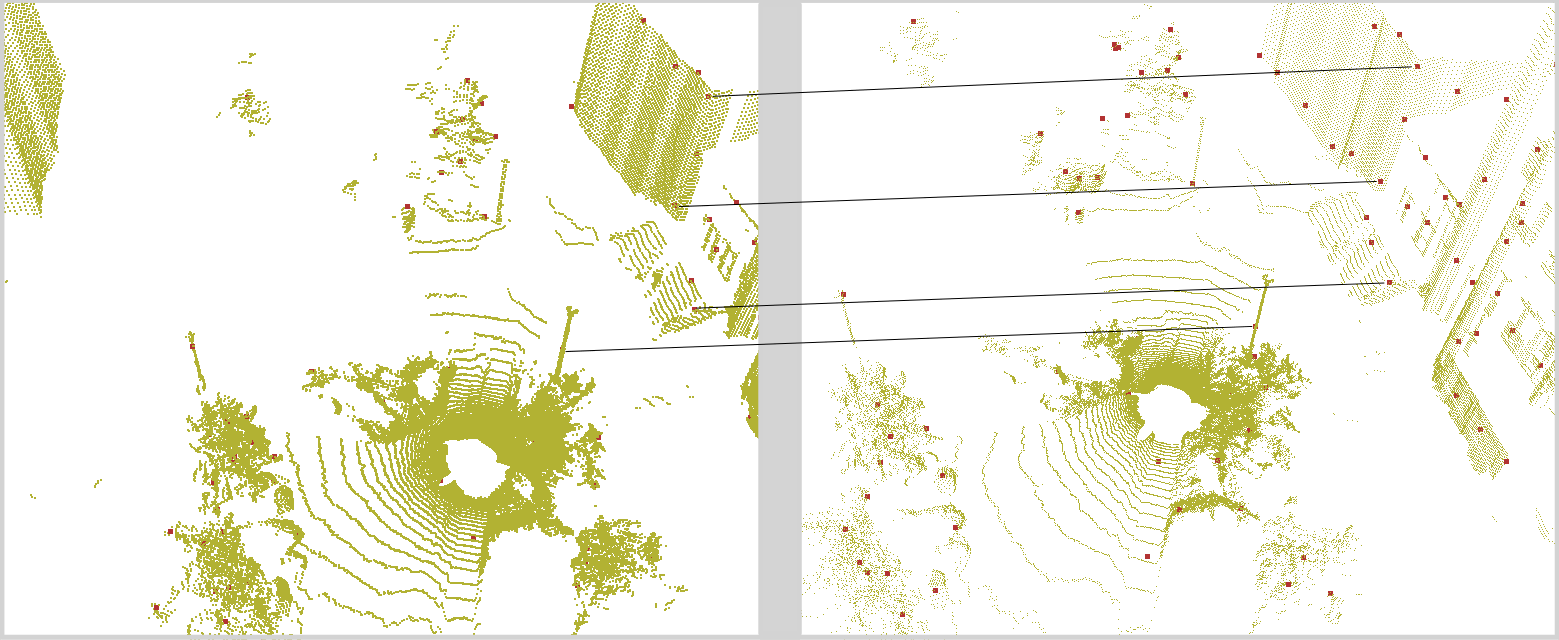
\includegraphics[width=0.995\linewidth]{img/chap_slam/features_line.png}\\
    \caption{Examples of NARF keypoints found for two different scans of the structured dataset. Black lines illustrate examples of valid correspondences found. These show stability under changes, such as viewpoint, noise and resolution.}
    \label{fig:chap_slam_features_correspondences}
\end{figure}


\subsection{Overview of the Algorithm}
\label{ssec:chap_slam_algo}

The original version of the place recognition algorithm was presented in~\cite{Steder2010}. It uses features correspondences to find valid transformations between all pairs of scans. Using a series of rules, a score is assigned to each transformation. This score reflects the system belief of this transformation to be an actual match. Although this technique yield high recognition rates, it requires a lot of processing time. An enhanced version of the algorithm, that we used for our experiments, was presented in~\cite{Steder2011b}. To improve processing time, they select only pairs of scans with the highest \gls*{bow} similarity for the scoring step. Also, because the first version of the algorithm yield poor result in area with less distinctive structure, they added a self-similarity analysis. Using the score of the best non-identity transformation of a scan with respect to itself, they adjust the score with respect to the other scans, thereby reducing the number of false positive. Finally, they use the NARF features, which benefit from a rotation invariance parameter. Algorithm~\ref{alg:chap_slam_overview} present a high level pseudocode of the general scan matching process. Note that for the experiments, we used a \textit{C++} implementation developed by Bastian Steder.

In Algorithm~\ref{alg:chap_slam_overview}, NARF features are computed twice for each scan. The \gls*{bow} preprocessing from line~\ref{alg:bow_beginning} to~\ref{alg:bow_end} uses a set of feature parameters while the correspondences scoring from line~\ref{alg:correspondences_beginning} to line~\ref{alg:correspondences_end} use a different set of parameters. Table~\ref{tab:chap_slam_narf_parameters} shows the feature parameters used for those two cases. Authors explain that: \enquote{For the BoW approach a high number of features describing small parts of the environment is most useful\dots However, when matching a new query [scan] $z*$ against D [the database], a smaller number of more distinctive features is needed}.

The first produced descriptors are used by the \textsc{createDictionaryForBagOfWord} function, which create 200 words (i.e clusters) using k-means. The output dictionary is used to create a \gls*{bow} representation for each scan. Based on this representation, all scans from the database are stored in ascending order, according to their Euclidean distance from the input scan (line~\ref{alg:init_similarities}). Scans with a small distance between them are more likely to originate from the same place and will be processed first during the next step. This order is important because of the timeout (line~\ref{alg:timeout}) that might prevent last scans to be processed.

The features created using the second set of parameters are used to find potential transformations between each database scan and the input scan. Since each NARF feature encodes its 3D pose, a single features match allows to determine the transformation between the two scans. Therefore, there is up to 2000 transformations to be tested for each scan from the database. To determine the corresponding features, all pairs of features (one from the processed database scan and one from the input scan) are then ordered by ascending order according to their Manhattan distance in the space of descriptors. Again, descriptors with a small distance between them are more similar and therefore more likely to be valid matches.

Although the transformation scoring algorithm is not detailed in Algorithm~\ref{alg:chap_slam_overview}, it is an important part of the place recognition framework that we will briefly describe here.
\begin{itemize}
    \item given a model of our sensor
    \item from the sensor’s origin along a line to the measured point
    \item Validation point from the query scan
    \item we can calculate the pixel position p in the range image of zk in which the point p would fall into as well as the range value r the point should have.
    \item we will now calculate a score and a weight reflecting how good the r prediction is explained by the observation
\end{itemize}
They then give a score following a predefined procedure for every possible cases:
\begin{itemize}
    \item The observation is within a confidence interval, therefore representing blabla.
    \item The observed range is larger than the predicted one
    \item The observed range is smaller than the predicted range
    \item The point is unobserved in the database range image
    \item The point is a far range reading in the range image from the database
\end{itemize}
The final score is a function of all points computed for the match. 
To avoid a small error in the transformation to cause low score, they also consider neighbors in small pixel radius.
They dont do it on all points of the scans (it would be too long), but rather use a subsample of points that better cover the 3D space.

\begin{algorithm}
    \begin{algorithmic}[1]
        \INPUT
        \Statex $scanDatabase$ : the complete database of previous scans (range images)
        \Statex $newScan$ : the new scan to be processed
        \OUTPUT
        \Statex $potentialMatches$ : set of (scanDatabase potential match for the newScan, best relative transformation, transformation score)
        \Statex

        \Function{findPotentialMatches}{$scanDatabase$, $newScan$}
        \State $allBowDescriptors \gets \textsc{calculateAllDescriptorsForBagOfWords}(scanDatabase)$ \label{alg:bow_beginning}
        \State $dictionary \gets \textsc{createDictionaryForBagOfWords}(allBowDescriptors)$
        \State $newScanBow \gets \textsc{computeBagOfWords}(newScan, dictionary)$ \Comment{Keep scan reference} \label{alg:create_bow}
        \State \State $initSimilarities \gets \emptyset$ \Comment{Set of (scan reference, initial similarity score)}
        \ForAll{$scan \in scanDatabase$}
        \State $scanBow \gets \textsc{computeBagOfWords}(scan, dictionary)$
        \State $initSimilarities.append(\textsc{getInitSimilarity}(scanBow, newScanBow))$ \label{alg:init_similarities}
        \EndFor
        \State $sortedSimilarities \gets \textsc{sortByScore}(initSimilarities)$ \label{alg:bow_end}

        \State
        \State $potentialMatches \gets \emptyset$, $i \gets 1$ \label{alg:correspondences_beginning}
        \State $newScanFeatures \gets \textsc{getScanFeatures}(newScan)$  \Comment{Each feature encodes the 3D pose} \label{alg:features_1}
        \While{$time \leq timeout$ \textbf{and} $i \leq |scanDatabase|$} \label{alg:timout}
        \State $scan \gets \textsc{getScan}(sortedSimilarities_i)$
        \State $scanFeatures \gets \textsc{getScanFeatures}(scan)$ \Comment{Each feature encodes the 3D pose} \label{alg:features_2}
        \State $sortedMatches \gets \textsc{getSortedFeatureMatches}(scanFeatures, newScanFeatures)$ \label{alg:ordered_matches}

        \State
        \State $j \gets 1$, $bestTransfoScore = -\infty$, $bestTransfo \gets null$
        \While{$j \leq |sortedMatches|$ \textbf{and} $j \leq 2000$} 
        \State $transfo,score \gets \textsc{computeMatchTransfoAndScore}(sortedMatches_j)$
        \If{$score \geq scoreAcceptanceThreshold$ \textbf{and} $score \geq bestTransfoScore$}
        \State $bestTransfoScore \gets score$
        \State $bestTransfo \gets transfo$
        \EndIf
        \State $j \gets j + 1$
        \EndWhile

        \State
        \If{$bestTransfo \neq null$}
        \State $potentialMatches.append(scan, bestTransfo, bestTransfoScore)$
        \EndIf

        \State
        \State $i \gets i+1$
        \EndWhile \label{alg:correspondences_end}

        \State
        \State \Return{$potentialMatches$}
        \EndFunction
    \end{algorithmic}

    \caption{High Level Place Recognition Process}
    \label{alg:chap_slam_overview}
\end{algorithm}

\begin{table}[H]
    \centering
    \begin{tabular}{@{}lll@{}}
        \toprule
        \textbf{Parameter}  & \textbf{Value for \gls*{bow}} & \textbf{Value for correspondences} \\
        \hline
        Max. feature counts & 2000                          & 200                                \\
        Descriptor size     & 36                            & 36                                 \\
        Support size        & 1/10 avg. range               & 1/5 avg. range                     \\
        \bottomrule
    \end{tabular}
    \caption{\todo{}}
    \label{tab:chap_slam_narf_parameters}
\end{table}

